
\section{Frequenzzuteilung}
\label{section:frequenzzuteilung}
\begin{frame}%STARTCONTENT
\begin{itemize}
  \item Jede Frequenznutzung bedarf einer vorherigen \emph{Frequenzzuteilung}
  \item Verankert im Telekommunikationsgesetz (TKG)
  \item Einzelzuteilung oder Allgemeinzuteilung
  \end{itemize}

\end{frame}

\begin{frame}\begin{itemize}
  \item Amateurfunk darf nur auf den zugeteilten Frequenzen durchgeführt werden
  \item Frequenzbereiche sind zwar international vereinbart
  \item \emph{Aber} die nationalen Bestimmungen sind maßgebend
  \end{itemize}
\end{frame}

\begin{frame}
\only<1>{
\begin{QQuestion}{VE102}{Bedarf jede Frequenznutzung einer Frequenzzuteilung?}{Eine Frequenznutzung ist auch ohne Frequenzzuteilung zulässig.}
{Erst ab \qty{0,1}{\W} ist eine Frequenzzuteilung erforderlich.}
{Es gibt Ausnahmen von der Notwendigkeit zur Frequenzzuteilung, z.~B. die ISM-Frequenzen.}
{Jede Frequenznutzung bedarf einer vorherigen Frequenzzuteilung.}
\end{QQuestion}

}
\only<2>{
\begin{QQuestion}{VE102}{Bedarf jede Frequenznutzung einer Frequenzzuteilung?}{Eine Frequenznutzung ist auch ohne Frequenzzuteilung zulässig.}
{Erst ab \qty{0,1}{\W} ist eine Frequenzzuteilung erforderlich.}
{Es gibt Ausnahmen von der Notwendigkeit zur Frequenzzuteilung, z.~B. die ISM-Frequenzen.}
{\textbf{\textcolor{DARCgreen}{Jede Frequenznutzung bedarf einer vorherigen Frequenzzuteilung.}}}
\end{QQuestion}

}
\end{frame}

\begin{frame}
\only<1>{
\begin{QQuestion}{VD701}{Darf ein Funkamateur in Deutschland alle in den Radio Regulations (RR) für den Amateurfunkdienst zugewiesenen Frequenzbereiche benutzen?}{Nein, es dürfen nur Frequenzen genutzt werden, die durch nationale Regelungen umgesetzt wurden.}
{Ja, weil die internationalen Regelungen der Radio Regulations (RR) auch in Deutschland gelten.}
{Ja, wenn der Betrieb bei der Bundesnetzagentur vorher angemeldet wurde.}
{Nein, die in Deutschland zulässigen Frequenzbereiche ergeben sich aus der Frequenznutzungsplanaufstellungsverordnung.}
\end{QQuestion}

}
\only<2>{
\begin{QQuestion}{VD701}{Darf ein Funkamateur in Deutschland alle in den Radio Regulations (RR) für den Amateurfunkdienst zugewiesenen Frequenzbereiche benutzen?}{\textbf{\textcolor{DARCgreen}{Nein, es dürfen nur Frequenzen genutzt werden, die durch nationale Regelungen umgesetzt wurden.}}}
{Ja, weil die internationalen Regelungen der Radio Regulations (RR) auch in Deutschland gelten.}
{Ja, wenn der Betrieb bei der Bundesnetzagentur vorher angemeldet wurde.}
{Nein, die in Deutschland zulässigen Frequenzbereiche ergeben sich aus der Frequenznutzungsplanaufstellungsverordnung.}
\end{QQuestion}

}
\end{frame}

\begin{frame}
\only<1>{
\begin{QQuestion}{VC110}{Was gilt für Funkamateure hinsichtlich der Frequenznutzung? Ein Funkamateur darf mit seiner Amateurfunkstelle~...}{beliebige Frequenzen nutzen, sofern keine anderen Funkdienste gestört werden.}
{auf allen für seine ITU-Region zugelassenen Frequenzen senden.}
{auf den für den Amateurfunkdienst ausgewiesenen Frequenzen senden.}
{im Rahmen einer Notfunkübung auch auf nicht für den Amateurfunkdienst ausgewiesenen Frequenzen senden.}
\end{QQuestion}

}
\only<2>{
\begin{QQuestion}{VC110}{Was gilt für Funkamateure hinsichtlich der Frequenznutzung? Ein Funkamateur darf mit seiner Amateurfunkstelle~...}{beliebige Frequenzen nutzen, sofern keine anderen Funkdienste gestört werden.}
{auf allen für seine ITU-Region zugelassenen Frequenzen senden.}
{\textbf{\textcolor{DARCgreen}{auf den für den Amateurfunkdienst ausgewiesenen Frequenzen senden.}}}
{im Rahmen einer Notfunkübung auch auf nicht für den Amateurfunkdienst ausgewiesenen Frequenzen senden.}
\end{QQuestion}

}
\end{frame}

\begin{frame}
\frametitle{Frequenzbereiche für den Amateurfunkdienst}
\begin{itemize}
  \item Sind in Deutschland in der Anlage 1 der \emph{Verordnung über den Amateurfunk (AFuV)} geregelt
  \item Senden nur auf den der Zeugnisklasse zugewiesenen Frequenzen
  \item Weitere einzuhaltende Nutzungsbestimmungen
  \item Es gibt ergänzende bindende Verfügungen und Mitteilungen
  \item Werden im Amtsblatt und auf der Webseite der Bundesnetzagentur (BNetzA) veröffentlicht
  \end{itemize}
\end{frame}

\begin{frame}
\begin{figure}
    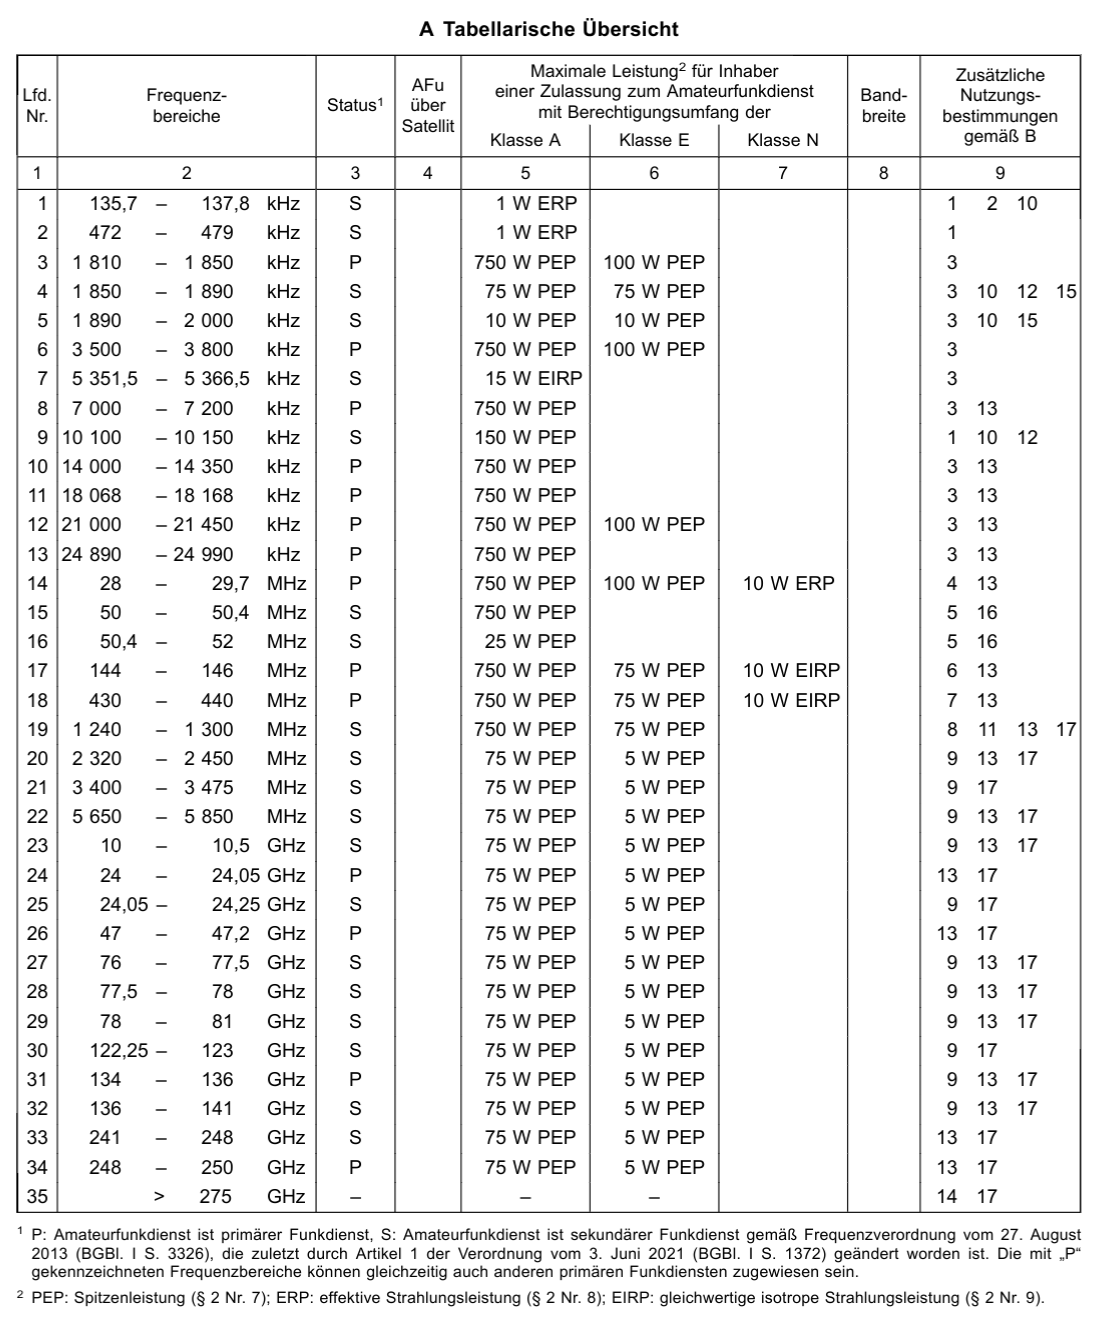
\includegraphics[width=0.85\textwidth]{foto/99}
    \caption{\scriptsize Tabellarische Übersicht, Anlage 1, AFuV (Korrektur in den Leistungen für Klasse~N notwendig)}
    \label{n_frequenzbereiche_afuv_anlage_1}
\end{figure}

\end{frame}

\begin{frame}
\only<1>{
\begin{QQuestion}{VD101}{Wo kann der Funkamateur nachschlagen, welche Frequenzbereiche er entsprechend seiner Zeugnisklasse in Deutschland nutzen darf?}{In der Anlage zur Frequenzverordnung (FreqV) und den dazugehörigen Mitteilungen der BNetzA}
{In den Radio Regulations (RR)}
{Im Amateurfunkgesetz (AFuG)}
{In der Anlage 1 der Amateurfunkverordnung (AFuV) und ggf. weiteren Mitteilungen der BNetzA}
\end{QQuestion}

}
\only<2>{
\begin{QQuestion}{VD101}{Wo kann der Funkamateur nachschlagen, welche Frequenzbereiche er entsprechend seiner Zeugnisklasse in Deutschland nutzen darf?}{In der Anlage zur Frequenzverordnung (FreqV) und den dazugehörigen Mitteilungen der BNetzA}
{In den Radio Regulations (RR)}
{Im Amateurfunkgesetz (AFuG)}
{\textbf{\textcolor{DARCgreen}{In der Anlage 1 der Amateurfunkverordnung (AFuV) und ggf. weiteren Mitteilungen der BNetzA}}}
\end{QQuestion}

}
\end{frame}

\begin{frame}
\only<1>{
\begin{QQuestion}{VD702}{Wo sind die für den Amateurfunkdienst in Deutschland ausgewiesenen Frequenzbereiche und die zugehörigen ausführlichen Nutzungsbedingungen zu finden?}{In Artikel~5 der Radio Regulations (RR)}
{In der Anlage 1 der Amateurfunkverordnung (AFuV) und ggf. weiteren Mitteilungen der BNetzA}
{Im Frequenzplan (FreqP)}
{In der Anlage zur Frequenzverordnung (FreqV)}
\end{QQuestion}

}
\only<2>{
\begin{QQuestion}{VD702}{Wo sind die für den Amateurfunkdienst in Deutschland ausgewiesenen Frequenzbereiche und die zugehörigen ausführlichen Nutzungsbedingungen zu finden?}{In Artikel~5 der Radio Regulations (RR)}
{\textbf{\textcolor{DARCgreen}{In der Anlage 1 der Amateurfunkverordnung (AFuV) und ggf. weiteren Mitteilungen der BNetzA}}}
{Im Frequenzplan (FreqP)}
{In der Anlage zur Frequenzverordnung (FreqV)}
\end{QQuestion}

}
\end{frame}%ENDCONTENT
